\documentclass{beamer}
\mode<presentation>{
  \usetheme{Boadilla}
  \usefonttheme[onlylarge]{structurebold}
  \usefonttheme[stillsansseriflarge]{serif}
  \setbeamerfont*{frametitle}{size=\normalsize,series=\bfseries}
  % \setbeamertemplate{navigation symbols}{}
  \setbeamercovered{transparent}
}
\usepackage[english]{babel}
\usepackage[latin1]{inputenc}
\usepackage{times}
\usepackage[T1]{fontenc}
\usepackage{amsmath}
\usepackage{amssymb}
\usepackage{esint}
\usepackage{hyperref}
\usepackage{tikz}
\usepackage{xkeyval}
\usepackage{xargs}
\usepackage{verbatim}
\usepackage{listings}
\usepackage{multimedia}
\usetikzlibrary{
  arrows,
  calc,
  decorations.pathmorphing,
  decorations.pathreplacing,
  decorations.markings,
  fadings,
  positioning,
  shapes
}

\mode<handout>{
  \usepackage{pgfpages}
  \pgfpagesuselayout{4 on 1}[a4paper,landscape,border shrink=5mm]
  \setbeamercolor{background canvas}{bg=black!10}
}

\newcommand\pgfmathsinandcos[3]{%
  \pgfmathsetmacro#1{sin(#3)}%
  \pgfmathsetmacro#2{cos(#3)}%
}
\newcommand\LongitudePlane[3][current plane]{%
  \pgfmathsinandcos\sinEl\cosEl{#2} % elevation
  \pgfmathsinandcos\sint\cost{#3} % azimuth
  \tikzset{#1/.estyle={cm={\cost,\sint*\sinEl,0,\cosEl,(0,0)}}}
}
\newcommand\LatitudePlane[3][current plane]{%
  \pgfmathsinandcos\sinEl\cosEl{#2} % elevation
  \pgfmathsinandcos\sint\cost{#3} % latitude
  \pgfmathsetmacro\yshift{\cosEl*\sint}
  \tikzset{#1/.estyle={cm={\cost,0,0,\cost*\sinEl,(0,\yshift)}}} %
}
\newcommand\DrawLongitudeCircle[2][1]{
  \LongitudePlane{\angEl}{#2}
  \tikzset{current plane/.prefix style={scale=#1}}
  % angle of "visibility"
  \pgfmathsetmacro\angVis{atan(sin(#2)*cos(\angEl)/sin(\angEl))} %
  \draw[current plane] (\angVis:1) arc (\angVis:\angVis+180:1);
  \draw[current plane,dashed] (\angVis-180:1) arc (\angVis-180:\angVis:1);
}
\newcommand\DrawLatitudeCircleArrow[2][1]{
  \LatitudePlane{\angEl}{#2}
  \tikzset{current plane/.prefix style={scale=#1}}
  \pgfmathsetmacro\sinVis{sin(#2)/cos(#2)*sin(\angEl)/cos(\angEl)}
  % angle of "visibility"
  \pgfmathsetmacro\angVis{asin(min(1,max(\sinVis,-1)))}
  \draw[current plane,decoration={markings, mark=at position 0.6 with {\arrow{<}}},postaction={decorate},line width=.6mm] (\angVis:1) arc (\angVis:-\angVis-180:1);
  \draw[current plane,dashed,line width=.6mm] (180-\angVis:1) arc (180-\angVis:\angVis:1);
}
\newcommand\DrawLatitudeCircle[2][1]{
  \LatitudePlane{\angEl}{#2}
  \tikzset{current plane/.prefix style={scale=#1}}
  \pgfmathsetmacro\sinVis{sin(#2)/cos(#2)*sin(\angEl)/cos(\angEl)}
  % angle of "visibility"
  \pgfmathsetmacro\angVis{asin(min(1,max(\sinVis,-1)))}
  \draw[current plane] (\angVis:1) arc (\angVis:-\angVis-180:1);
  \draw[current plane,dashed] (180-\angVis:1) arc (180-\angVis:\angVis:1);
}
\newcommand\coil[1]{
  {\rh * cos(\t * pi r)}, {\apart * (2 * #1 + \t) + \rv * sin(\t * pi r)}
}
\makeatletter
\define@key{DrawFromCenter}{style}[{->}]{
  \tikzset{DrawFromCenterPlane/.style={#1}}
}
\define@key{DrawFromCenter}{r}[1]{
  \def\@R{#1}
}
\define@key{DrawFromCenter}{center}[(0, 0)]{
  \def\@Center{#1}
}
\define@key{DrawFromCenter}{theta}[0]{
  \def\@Theta{#1}
}
\define@key{DrawFromCenter}{phi}[0]{
  \def\@Phi{#1}
}
\presetkeys{DrawFromCenter}{style, r, center, theta, phi}{}
\newcommand*\DrawFromCenter[1][]{
  \setkeys{DrawFromCenter}{#1}{
    \pgfmathsinandcos\sint\cost{\@Theta}
    \pgfmathsinandcos\sinp\cosp{\@Phi}
    \pgfmathsinandcos\sinA\cosA{\angEl}
    \pgfmathsetmacro\DX{\@R*\cost*\cosp}
    \pgfmathsetmacro\DY{\@R*(\cost*\sinp*\sinA+\sint*\cosA)}
    \draw[DrawFromCenterPlane] \@Center -- ++(\DX, \DY);
  }
}
\newcommand*\DrawFromCenterText[2][]{
  \setkeys{DrawFromCenter}{#1}{
    \pgfmathsinandcos\sint\cost{\@Theta}
    \pgfmathsinandcos\sinp\cosp{\@Phi}
    \pgfmathsinandcos\sinA\cosA{\angEl}
    \pgfmathsetmacro\DX{\@R*\cost*\cosp}
    \pgfmathsetmacro\DY{\@R*(\cost*\sinp*\sinA+\sint*\cosA)}
    \draw[DrawFromCenterPlane] \@Center -- ++(\DX, \DY) node {#2};
  }
}
\makeatother

% not mandatory, but I though it was better to set it blank
\setbeamertemplate{headline}{}
\def\beamer@entrycode{\vspace{-\headheight}}

\tikzstyle{snakearrow} = [decorate, decoration={pre length=0.2cm,
  post length=0.2cm, snake, amplitude=.4mm,
  segment length=2mm},thick, ->]

%% document-wide tikz options and styles

\tikzset{%
  % >=latex, % option for nice arrows
  inner sep=0pt,%
  outer sep=2pt,%
  mark coordinate/.style={inner sep=0pt,outer sep=0pt,minimum size=3pt,
    fill=black,circle}%
}
\tikzset{
  % Define standard arrow tip
  >=stealth',
  % Define style for boxes
  punkt/.style={
    rectangle,
    rounded corners,
    draw=black, very thick,
    text width=8em,
    minimum height=2.5em,
    text centered},
}
\makeatletter
\newbox\@backgroundblock
\newenvironment{backgroundblock}[2]{%
  \global\setbox\@backgroundblock=\vbox\bgroup%
  \unvbox\@backgroundblock%
  \vbox to0pt\bgroup\vskip#2\hbox to0pt\bgroup\hskip#1\relax%
}{\egroup\egroup\egroup}
\addtobeamertemplate{background}{\box\@backgroundblock}{}
\makeatother

% \def\timeleft{15:00->14:55}

\title{Apparatus for making dipolar NaCs molecules}
\author{Yichao Yu}
\institute{Ni Group/Harvard}

\begin{document}

% Goal of our experiment:
%
% Develop a new approach to make dipolar di-atomic molecules with single
% site addressability.
% As a platform for quantum simulation/computing, quantum chemistry etc.

% Method (illustrated in the picture) we use
% 1. MOT
% 2. Trap single atom in optical dipole trap
% 3. Raman sideband cooling
% 4. STIRAP to molecular ground state

\begin{frame}{}
  % TODO figure
  \titlepage
\end{frame}

% Currently we've got
% PIC: Cs single atom
% PIC: Cs Raman sideband
% PIC: Na MOT

% As one can tell. Soldium is harder. Apart from expected reasons like
% the properties of the atom. Also laser

\begin{frame}{Current state}
  \begin{block}{}
    % TODO pictures
    \begin{itemize}[<+->]
    \item Trapping Cs single atom
    \item Cs single atom cooling
    \item Na MOT
    \item Looking for trapped single Na atom
    \end{itemize}
  \end{block}
  \visible<+->{
    \begin{block}{Problems}
      \begin{itemize}[<+->]
      \item Sodium laser
      \item MOT stability
      \end{itemize}
    \end{block}
  }
\end{frame}

% Since we are using Na, need sodium laser
% Frequencies

% As usual also requires
% * Narrow linewidth
% * Tunable
% * (Low cost)

% Use diode
% * Cheap
% * Compact
% * Everyone knows how to use it

% Gap around the frequency we want
% Frequency doubling
% Bare diode cannot generate enough power
% Innolume diode (TODO: Picture)
% * Tunable over ~100nm (TODO: Test data)
% * High power (TODO: Test data)
% Waveguide frequency doubler (TODO: Picture)
% * High effeciency (TODO: Test data)

\begin{frame}{Laser system for Sodium}
  \begin{columns}
    \column{5.8cm}
    \begin{block}{Sodium wavelengths}
      \begin{itemize}
      \item<1-> D lines $\approx589$nm
      \item<2-> D2 line (Cooling, Imaging)
      \item<3-> D1 line (Pumping, Cooling)
      \item<4-> Off resonance (Raman transition)
      \end{itemize}
    \end{block}
    \visible<6->{
      % TODO Sodium wavelength
      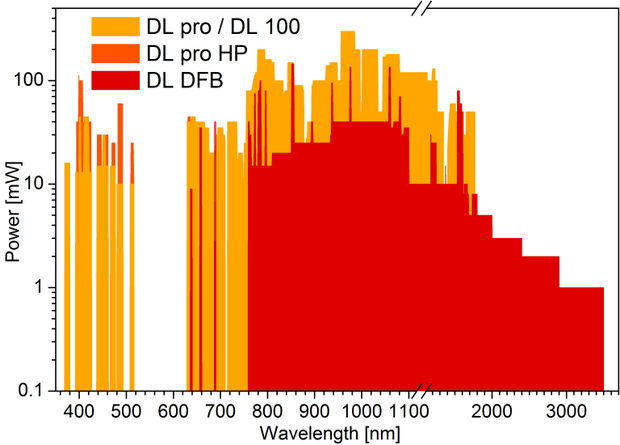
\includegraphics[width=5.5cm]{toptica_diode_spectrum.png}
    }
    \column{5.8cm}
    \only<5-> {
      \begin{block}{Using \only<7->{doubled }diode laser\only<7->{ $589\times2=1178$nm}}
        \begin{itemize}
        \item<6-> Diode laser spectrum
        \item<8-> Power requirement for frequency doubling
        \item<9-> Diode laser from Innolume / TimeBase\\
          \visible<10->{Tunable from $...$nm to $...$nm}
        \item<12-> Waveguide doubler
        \end{itemize}
      \end{block}
    }
  \end{columns}
\end{frame}

% Another problem: MOT stability
% Reason
% Small beam and small MOT (sensitive loading)
% multiple reflections / other fluctuations from glass plates (TODO: diagram)

% Modulating at high frequency (kHz) to average out any static effect
% (TODO: diagram)
% Video?

% Figures
% * Overall plan
% * Organize pictures with timeline
% * Cs single atom
% * Cs Raman sideband
% * Na MOT
% * Innolume diode
% * Innolume frequency tuning range
% * Innolume power
% * Doubler
% * Doubler effeciency
% * Setup

\begin{frame}{MOT stability}
  \begin{itemize}[<+->]
  \item Interference and stability issue with a small MOT
  \item Modulating the MOT beams
  \end{itemize}
\end{frame}

\begin{frame}{Members}
\end{frame}

\end{document}
